% EarRepair -- PerCom 2027 Work-in-Progress submission.
% Limit: 4 pages INCLUDING references, IEEE two-column, US letter, single-blind (authors shown).
%
% Numbers: every participant result comes from results.tex, written by
%   python analysis/analyze.py data/ --latex paper/results.tex
% Without results.tex the paper compiles as a design-and-system WiP with no results section.
% System numbers (clip durations, interaural cues) come from tests/test_app.py and the audio files.
\documentclass[conference,letterpaper]{IEEEtran}
\IEEEoverridecommandlockouts
% IEEEtran asks for Times. pdfLaTeX (Overleaf's default, and what IEEE expects) has it built in.
% XeTeX/Tectonic does not, so use the TeX Gyre Termes clone there. pdfLaTeX output is unchanged.
\usepackage{iftex}
\ifXeTeX
  \usepackage{fontspec}
  \setmainfont{texgyretermes}[Extension=.otf, UprightFont=*-regular, BoldFont=*-bold,
    ItalicFont=*-italic, BoldItalicFont=*-bolditalic]
\fi
\usepackage{cite}
\usepackage{amsmath}
\usepackage{graphicx}
\usepackage{booktabs}
\usepackage{xcolor}
\usepackage{tikz}
\usetikzlibrary{positioning}
\usepackage[hidelinks]{hyperref}

\newcommand{\todo}[1]{\textcolor{red}{[TODO: #1]}}
\newif\ifhaveresults
\IfFileExists{results.tex}{\input{results.tex}}{}
% Fallback for every number that results.tex provides. \providecommand never overrides a real value,
% so after `analyze.py --latex paper/results.tex` these are unused. Without results.tex the results
% section is switched off (\ifhaveresults is false), so none of these appear in the PDF.
\newcommand{\phx}{\textcolor{red}{??}}
\providecommand{\resN}{\phx}
\makeatletter
\@for\m:={Time,Acc,Tlx,Walk}\do{%
  \@for\c:={Numbered,Plain,Spatial}\do{%
    \expandafter\providecommand\csname res\m\c\endcsname{\phx}%
    \expandafter\providecommand\csname res\m Sd\c\endcsname{\phx}}%
  \@for\c:={Numbered,Plain}\do{%
    \expandafter\providecommand\csname res\m Vs\c\endcsname{\phx}%
    \expandafter\providecommand\csname res\m Ci\c\endcsname{\phx}%
    \expandafter\providecommand\csname res\m P\c\endcsname{\phx}%
    \expandafter\providecommand\csname res\m Dz\c\endcsname{\phx}}}
\makeatother


\begin{document}

\title{EarRepair: Spatial Audio for Eyes-Free Correction\\ of Misrecognised Voice Commands}

% Single-blind: real names and affiliations are required.
\author{\IEEEauthorblockN{\todo{Author names}}
\IEEEauthorblockA{\todo{Department, institution, city, country}\\
\todo{email addresses}}}

\maketitle

\begin{abstract}
When a voice assistant is unsure which contact a user meant, the usual repair asks the user to look at
the phone, repeat the name, or listen to a numbered list of alternatives. All three are awkward while
walking. We present EarRepair, which plays the assistant's candidate contacts at distinct positions
around the listener through ordinary earphones, so that the user picks one with a single eyes-free
swipe towards it. We describe the technique, a browser-based prototype, and a within-subjects walking
study that compares spatial presentation with a numbered spoken list and with a plain list. The plain
list separates the effect of position from the time the numbers add, which is 35\% of the list.
\ifhaveresults
In a pilot with \resN{} participants, \todo{one-sentence summary of the main result, written after the analysis}.
\else
We report the design rationale, the measured spatial cues of the prototype, and the analysis plan of
the ongoing study.
\fi
\end{abstract}

\begin{IEEEkeywords}
spatial audio, voice assistants, error repair, eyes-free interaction, earables
\end{IEEEkeywords}

\section{Introduction}
Earphones are now an always-worn interface to a pervasive assistant~\cite{roddiger2022sensing}. A
common request through them is ``Call Riya''. Proper names remain hard for speech recognisers, which
is why contextual biasing towards a user's own entities is an active topic~\cite{zhao2019shallow}.
When recognition is uncertain, the assistant has a few plausible matches, for example
\emph{Riya Shah}, \emph{Rina Rao} and \emph{Priya Sharma}, and the user has to repair the request.

Today's repairs fit poorly on the move. Looking at the phone breaks the eyes-free use that earphones
afford. Repeating the name invites another recognition error, especially in noise, and users already
fall back on repetition and rephrasing when voice interfaces fail~\cite{myers2018patterns,
beneteau2019communication}. A spoken, numbered list of alternatives avoids both, but it is serial and
slow, and the user must hold the numbers in mind. Users do favour repairs in which the system offers
options~\cite{ashktorab2019resilient}. The open question is how to offer them without the screen.

EarRepair plays the candidates one after another from the left, the front and the right of the
listener. The user swipes towards the intended name, anywhere on the screen and without looking, as
soon as they hear it. Position replaces the number, so the list is shorter, and selecting becomes a
matter of pointing at where the name came from.

This work-in-progress paper contributes (1)~the EarRepair technique and an open, instrumented
prototype that runs in a phone browser, and (2)~a walking study design with two features that earlier
spatial-audio comparisons did not need: a plain-list control that separates the effect of position
from the duration of spoken numbers, and trials where the intended contact is not among the
candidates, as happens when recognition fails completely.

\section{Related Work}
\textbf{Repairing voice interactions.} Studies of everyday voice-interface use describe breakdowns as
routine, and repair as work that users do through repetition, rephrasing and changes in
prosody~\cite{porcheron2018voice,myers2018patterns,beneteau2019communication}. Suhm et al.\ showed that
correcting speech errors by switching modality, for example choosing from alternatives, can beat
respeaking~\cite{suhm2001multimodal}. Ashktorab et al.\ found that people prefer repair strategies in
which the system presents options~\cite{ashktorab2019resilient}. These works assume a screen, or a
spoken dialogue, to present the options. EarRepair keeps the options but moves them into space.

\textbf{Spatial and eyes-free auditory menus.} Brewster et al.\ placed menu items around the head and
selected them with head gestures. Egocentric sounds reduced task time and let users walk closer to
their preferred speed~\cite{brewster2003multimodal}. Lorho et al.\ used spatial separation to structure
hierarchical menus~\cite{lorho2002structured}. Vazquez-Alvarez and Brewster used spatial audio to
separate concurrent streams on mobile devices, and found that preferences between techniques reversed
under higher cognitive load~\cite{vazquez2010designing,vazquez2011eyesfree}. Eyes-free selection has
also used touch dials with reactive audio~\cite{zhao2007earpod}, free-hand gestures with auditory
menus~\cite{kajastila2013eyesfree}, and compressed speech cues that speed up menu
navigation~\cite{walker2013spearcons}. We are not aware of work that applies spatial presentation to
the specific, time-critical case of repairing an ambiguous voice command, where the user knows the
target and only needs to find it among a few similar-sounding names.

\textbf{Interaction while walking.} Walking degrades phone selection and reading
performance~\cite{schildbach2010walking}. Walking speed relative to a preferred-walking-speed baseline is
an established measure of the cost of mobile interaction~\cite{ng2014comparing}, which we adopt.

\section{EarRepair}
\textbf{Scenario.} The recogniser is simulated, so that every trial isolates the repair step. A trial
starts with the user's request (``Call Riya Shah'') in one voice. The assistant then asks ``Which one?''
in a second voice and plays three candidates. The user swipes left, up or right to choose, or down for
``none of these''. A tap replays the candidates, and a swipe is accepted from the moment the first
candidate starts, so experienced users can answer before the list ends.

\textbf{Spatial rendering.} Candidates play in a fixed order at $-90^{\circ}$, $0^{\circ}$ and
$+90^{\circ}$ azimuth through the Web Audio HRTF panner, so the technique needs only stereo earphones and
a browser. The order is fixed so that space adds to, rather than replaces, the order that a spoken list
already has. The two non-spatial conditions are rendered through the same panner at $0^{\circ}$, so the
voices are filtered identically in all conditions and only position differs. Measured at the ears, the
side positions differ by 3.2\,dB in level and about 0.79\,ms in arrival time, on the correct side, and
the front position is balanced. A generic HRTF is known to increase front--back
confusions~\cite{wenzel1993localization}. We therefore use only the frontal half-plane, and treat the
front position as the one to verify by ear before the study.

\textbf{Stimuli.} The 45 candidate triples use common Indian names, spoken by Indian-English synthetic
voices and normalised to equal loudness. In 24 triples the names sound alike (\emph{Neha Jain},
\emph{Neha Jha}, \emph{Nisha Jain}), as in a real recognition confusion. In 21 they are clearly distinct.
Fig.~\ref{fig:trial} shows the three ways the same candidates are presented.

\textbf{Prototype.} EarRepair runs as a single web page on the phone, with no installation
(Fig.~\ref{fig:screens}). During trials, the whole screen is a dark swipe surface with no names on it,
so there is nothing to read. The app logs every trial with millisecond timing on the audio clock,
corrected by the output latency that the browser reports. It saves after every trial, and repeats a trial
interrupted by a call or an app switch. An automated end-to-end test drives a full session in a
browser with emulated touch, including early, diagonal and interrupted gestures.

\begin{figure}[t]
\centering
% Each row is a chain of boxes placed right of the previous one, so nothing can overlap.
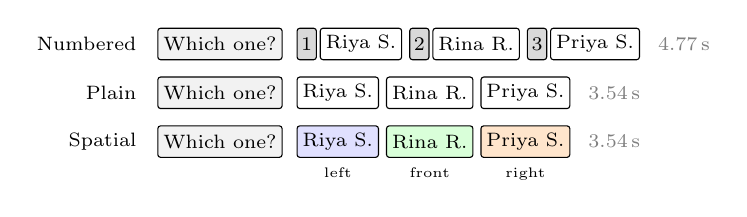
\begin{tikzpicture}[font=\scriptsize,node distance=2.5pt,
  box/.style={draw,rounded corners=1pt,minimum height=0.40cm,inner sep=2pt},
  ask/.style={box,fill=gray!10},
  num/.style={box,fill=gray!30,inner sep=1.5pt},
  nm/.style={box,fill=white}]
  % Numbered
  \node[anchor=east] (l1) at (0,0) {Numbered};
  \node[ask,right=4pt of l1] (w1) {Which one?};
  \node[num,right=5pt of w1] (n1) {1}; \node[nm,right=1pt of n1] (a1) {Riya S.};
  \node[num,right=of a1] (n2) {2};     \node[nm,right=1pt of n2] (b1) {Rina R.};
  \node[num,right=of b1] (n3) {3};     \node[nm,right=1pt of n3] (c1) {Priya S.};
  \node[right=3pt of c1,text=gray] {4.77\,s};
  % Plain
  \node[anchor=east] (l2) at (0,-0.62) {Plain};
  \node[ask,right=4pt of l2] (w2) {Which one?};
  \node[nm,right=5pt of w2] (a2) {Riya S.};
  \node[nm,right=of a2] (b2) {Rina R.};
  \node[nm,right=of b2] (c2) {Priya S.};
  \node[right=3pt of c2,text=gray] {3.54\,s};
  % Spatial
  \node[anchor=east] (l3) at (0,-1.24) {Spatial};
  \node[ask,right=4pt of l3] (w3) {Which one?};
  \node[nm,right=5pt of w3,fill=blue!12] (a3) {Riya S.};
  \node[nm,right=of a3,fill=green!15] (b3) {Rina R.};
  \node[nm,right=of b3,fill=orange!20] (c3) {Priya S.};
  \node[right=3pt of c3,text=gray] {3.54\,s};
  \node[below=0pt of a3,font=\tiny] {left};
  \node[below=0pt of b3,font=\tiny] {front};
  \node[below=0pt of c3,font=\tiny] {right};
\end{tikzpicture}
\caption{After the request, the same three candidates are presented in one of three ways. Only the cue
that marks each candidate differs: a spoken number, order alone, or position. In every condition the
user swipes $\leftarrow$, $\uparrow$ or $\rightarrow$ for the first, second or third candidate,
$\downarrow$ for none of these, and taps to replay. Grey figures are the mean list durations over all
45 items.}
\label{fig:trial}
\end{figure}

\begin{figure}[t]
\centering
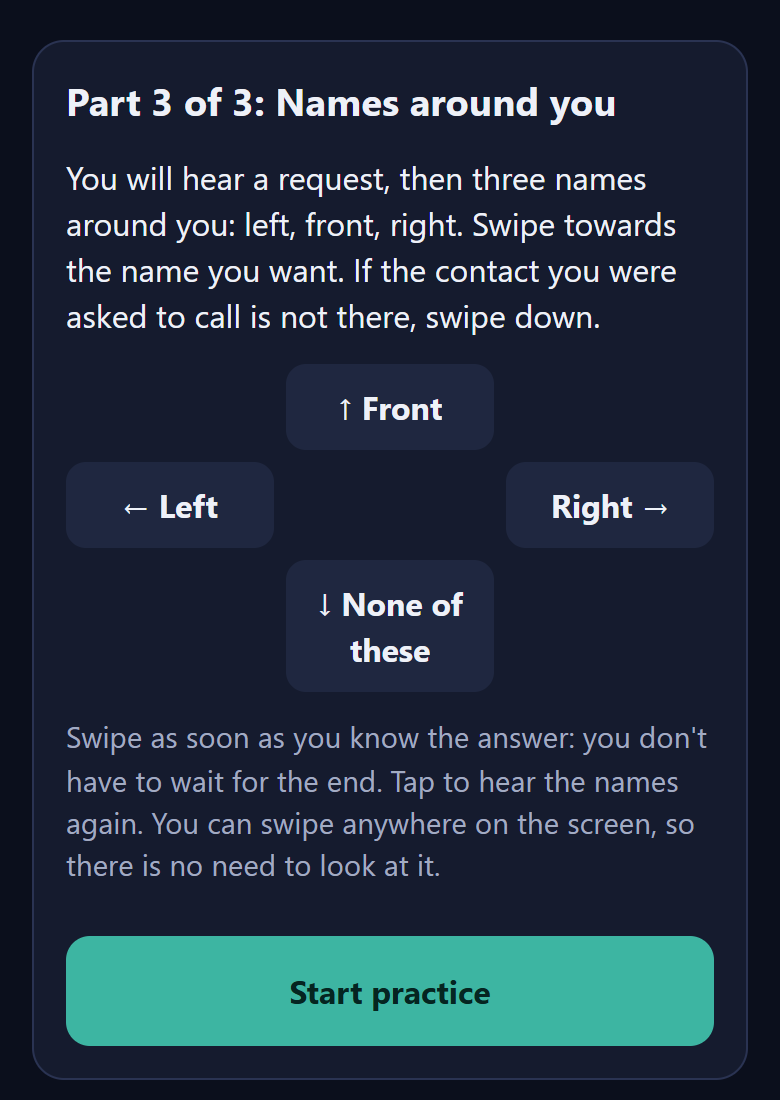
\includegraphics[width=0.47\columnwidth]{figs/screen_intro.png}\hfill
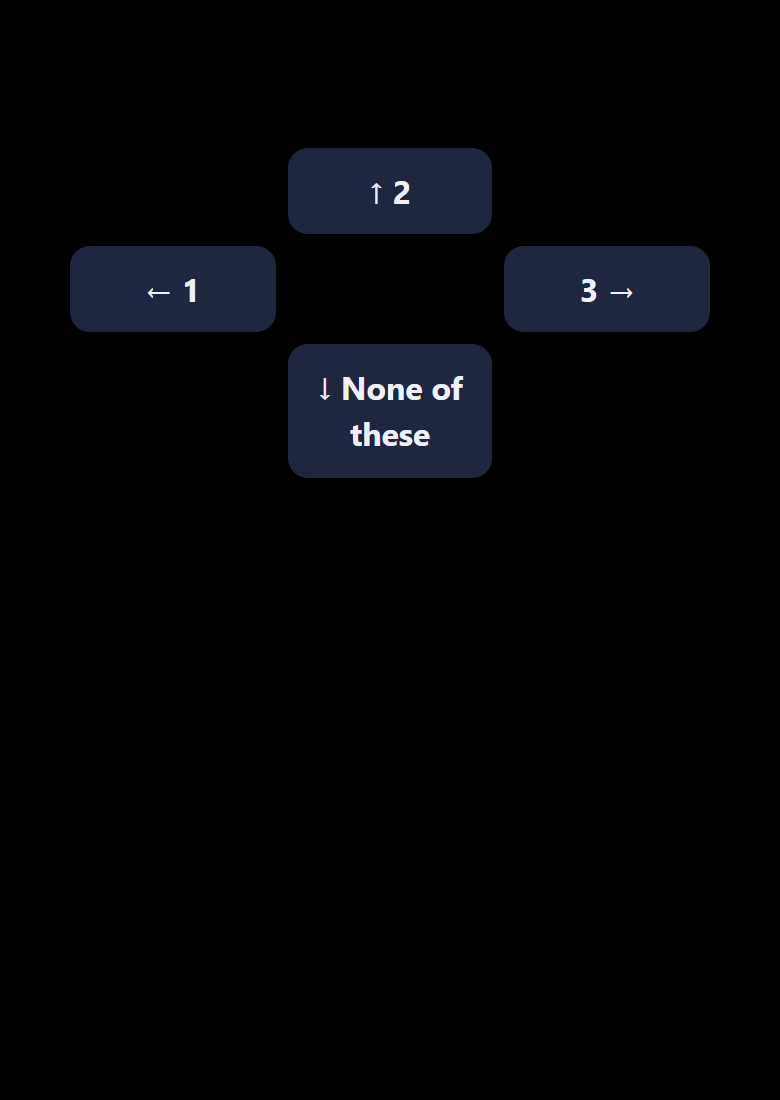
\includegraphics[width=0.47\columnwidth]{figs/screen_pad.png}
\caption{The prototype in a phone browser. Left: block instructions with the swipe legend for the
spatial condition. Right: the full-screen swipe surface during practice. In the measured trials the
legend is hidden as well, and the screen is black.}
\label{fig:screens}
\end{figure}

\section{Study Design}
\textbf{Conditions.} Three within-subject conditions present the candidates as (1)~a numbered list from
the front, the baseline that a voice assistant would use today; (2)~a plain list from the front; and
(3)~spatial positions. All use the same swipes. Numbers lengthen the list from 3.54\,s to 4.77\,s on
average (Fig.~\ref{fig:trial}). Comparing spatial with numbered therefore answers the practical
question, and comparing spatial with plain isolates the contribution of position.

\textbf{Hypotheses.} Stated before data collection: (H1)~spatial is faster than numbered; (H2)~spatial
is faster than plain, that is, position helps beyond a shorter list; (H3)~spatial is no less accurate
than either list, including on confusable names and absent contacts; and (H4)~spatial lowers rated
workload and costs less walking speed than numbered.

\textbf{Procedure.} Each participant first times one lap of a fixed indoor route without a task, to set
their preferred walking speed. After an earphone check (three correct left/right judgements in a row),
each condition is a block of 4 practice trials with feedback, followed by 15 trials while walking. The
15 trials contain 12 trials with the contact present, balanced over the three positions and over
confusable and distinct triples, and 3 with the contact absent. Condition order follows all six
permutations, and the three item sets rotate across conditions, so 12 participants cover every order
twice. After each block, participants rate their workload on the six raw NASA-TLX
scales~\cite{hart2006nasa}, and the experimenter records the laps walked. Participants finally name the
condition they liked most and least.

\textbf{Measures and analysis.} The primary measure is the time from the onset of the candidate list to
the finger touching the screen, on correct trials with the contact present. We also measure accuracy
(timeouts count as errors), replays, raw TLX, and walking speed as a share of the baseline. Each
participant contributes one median per condition. We compare spatial with numbered, and spatial with
plain, using exact sign-flip permutation tests with Holm correction and bootstrap 95\% confidence
intervals. These rules were fixed in the analysis script before any data were collected. With 10--15
participants, we treat the results as effect-size estimates for a larger study.

\ifhaveresults
\section{Preliminary Results}
\resN{} participants completed the study. Table~\ref{tab:results} summarises the per-participant means.
\todo{Describe the time, accuracy and TLX differences in one paragraph, using the numbers in the table.
Write the direction only as the data show it.}

\begin{table}[t]
\caption{Per-participant means (SD) by condition, and the paired difference from spatial with its
bootstrap 95\% CI and Holm-corrected $p$.}
\label{tab:results}
\centering
\scriptsize
\setlength{\tabcolsep}{3pt}
\begin{tabular}{@{}lccc@{}}
\toprule
 & Time (s) & Accuracy (\%) & Raw TLX \\
\midrule
Numbered & \resTimeNumbered{} (\resTimeSdNumbered) & \resAccNumbered{} (\resAccSdNumbered) & \resTlxNumbered{} (\resTlxSdNumbered) \\
Plain    & \resTimePlain{} (\resTimeSdPlain)       & \resAccPlain{} (\resAccSdPlain)       & \resTlxPlain{} (\resTlxSdPlain) \\
Spatial  & \resTimeSpatial{} (\resTimeSdSpatial)   & \resAccSpatial{} (\resAccSdSpatial)   & \resTlxSpatial{} (\resTlxSdSpatial) \\
\midrule
Spatial$-$Numbered & \resTimeVsNumbered & \resAccVsNumbered & \resTlxVsNumbered \\
\quad 95\% CI       & \resTimeCiNumbered & \resAccCiNumbered & \resTlxCiNumbered \\
\quad Holm $p$      & \resTimePNumbered  & \resAccPNumbered  & \resTlxPNumbered \\
Spatial$-$Plain    & \resTimeVsPlain    & \resAccVsPlain    & \resTlxVsPlain \\
\quad 95\% CI       & \resTimeCiPlain    & \resAccCiPlain    & \resTlxCiPlain \\
\quad Holm $p$      & \resTimePPlain     & \resAccPPlain     & \resTlxPPlain \\
\bottomrule
\end{tabular}
\end{table}
\fi

\section{Discussion and Next Steps}
\ifhaveresults
\todo{Interpret the pilot: does position help beyond a shorter list? Where were the errors? One paragraph.}
\else
Data collection with 12 participants is in progress. The study is built to tell apart two possible
explanations for a spatial benefit. If spatial is faster than numbered but not faster than plain, the
benefit comes from dropping the numbers, and a shorter spoken list would do as well. Only a difference
between spatial and plain shows that position itself helps. The error data add a second test: if
position is what users rely on, spatial errors should fall mostly on the neighbouring position, while
list errors should follow the order of the names.
\fi

\textbf{Limitations.} The recogniser is simulated, and the request names the full contact, so the
task is easier than recognising a contact from a vague memory. The voices are synthetic and band-limited
to 8\,kHz, which removes some of the spectral cues that separate front from back. The generic HRTF has
no head tracking, so the sounds turn with the head. A swipe still needs one free hand.

\textbf{Next steps.} We will (1)~add spoken selection (``the second one'') as a hands-free baseline,
(2)~use real recogniser confidence to decide when to offer a repair at all, (3)~add head tracking from
earphones that support it, so that candidates stay fixed in the world, and (4)~test in real street noise,
where a spoken repair is most likely to fail again.

\bibliographystyle{IEEEtran}
\bibliography{refs}

\end{document}
